\documentclass[12pt,a4paper]{article}
\usepackage[mag=1000, tikz]{newlistok}

\УвеличитьШирину{1.3cm}
\УвеличитьВысоту{2.3cm}
\renewcommand{\spacer}{\vspace{1.7pt}}

\ВключитьКолонтитул

\begin{document}

\Заголовок{Приложения основной теоремы арифметики}
\Оценки{35/30/25}
\НадНомеромЛистка{179 школа, 7Б.}
\НомерЛистка{15}
\ДатаЛистка{21.02 -- 10.03/2018}


\СоздатьЗаголовок

\задача
\пункт[Решето Эратосфена]
Выпишем целые числа от 2 до~$n$. Подчеркнём
2 и сотрём числа, кратные 2.
Первое неподчёркнутое число подчеркнём и сотрём %теперь
кратные ему, и т.~д.,
%Снова первое невычеркнутое число обведём в кружок, и т.~д.
%Будем действовать так,
пока каждое число от 2 до $n$
не будет подчёркнуто или стёрто.
Докажите, что мы подчеркнём в точности простые числа от~1~до~$n$.
\пункт  Пусть очередное число, которое мы хотим подчеркнуть, больше $\sqrt{n}$.
Докажите, что нестёртые к этому моменту числа от 2 до $n$ простые.
%натуральное число $a$, большее 1, не делится ни на одно простое число, меньшее $\sqrt{a}$. Докажите, что $a$ простое.
\пункт Какие числа, меньшие $100$, простые?
\кзадача

\задача  Числа $a$, $b$, $c$, $n$ натуральные, $(a,b)=1$, $ab=c^n$.
Найдется ли такое целое $x$, что~$a=x^n$?
%Верно ли, что $a=x^n$ %и $b=y^n$
%для некоторого целого $x$?
%натуральных чисел $x$ и $y$?
\кзадача

\пзадача
Решите в натуральных числах уравнение $x^{42}=y^{55}$.
\кзадача

\задача
Найдутся ли такие 10 разных целых чисел, ни одно из которых не квадрат целого числа, со свойством: квадратом целого числа будет
произведение
\пункт любых двух из них;
\пункт любых трёх них?
\кзадача


\пзадача
Найдите каноническое разложение числа \вСтрочку
\пункт 2018; \пункт 17!; \пункт $C_{20}^{10}$.
\кзадача

\задача
%\пункт
При каких натуральных $k$ число $(k-1)!$ не делится на $k$?
%\пункт При каких нечетных $n=2k+1$ число $k!+(k+1)\cdot\ldots\cdot(2k)$ не делится на $n$?
\кзадача



\ввпзадача
\вСтрочку
\пункт [Теорема Лежандра] Докажите, что простое число
$p$ входит в каноническое разложение числа $n!$
в степени $[n/p]+[n/p^2]+[n/{p^3}]+\dots$
(где $[x]$ --- это \выд{целая часть} числа $x$).
С какого момента слагаемые в этой сумме станут равными нулю?\\
\пункт Сколько у $2000!$ нулей в конце его десятичной записи?
% числа $2000!$?
\пункт Может ли $n!$ делиться на $2^n$ ($n\geq1$)?
\кзадача



\задача
Число $p$ простое. Докажите, что $C_p^k$ делится на
$p$, если $0<k<p$.
\кзадача

%\задача[Малая теорема Ферма]
%Докажите: $n^p-n$ делится на $p$, если $p$ ---
%простое,~\hbox{$n$ --- целое.}
%%Пусть $p$ простое.
%\кзадача

\ввпзадача[Малая теорема Ферма]
Пусть $p$ --- простое, $n$ --- целое.
\пункт Докажите индукцией по $n$, что $n^p-n$ делится на $p$.
\пункт  Докажите, что если $(n,p)=1$, то $n^{p-1}-1$ делится на $p$.
\кзадача


\ввпзадача Пусть $(a,p)=1$ и $p$ --- простое. \пункт Докажите, что
числа $a$, $2a$, \dots, $(p-1)a$ имеют разные ненулевые остатки от деления на $p$.
\пункт Выведите из пункта а) малую теорему Ферма.
\кзадача

\ввпзадача
Пусть $p$ простое. \пункт Докажите, что для каждого ненулевого остатка $a$ от деления на $p$ найдётся такой остаток $b$
от деления на $p$, что $ab\equiv 1 (\bmod p)$.
\пункт Для какиx $a$ из предыдущего пункта $b=a$?
\пункт[Критерий Вильсона] Докажите, что $(p-1)!+1$ делится на $p$.
\кзадача

% \сзадача
% \вСтрочку
% \пункт
% Числа $p$ и $q$ простые, $2^{p}-1\del q$. Докажите,
% что $q-1\del p$.
% \пункт
% Простое ли $2^{13}-1$?
% \кзадача


\сзадача Может ли быть целым число
\вСтрочку
\пункт
$\displaystyle{\frac{1}{2}+\frac{1}{3}+\frac{1}{4}+\ldots+\frac{1}{n}}$;
\пункт
$\displaystyle{\frac{1}{3}+\frac{1}{5}+\frac{1}{7}+\ldots+\frac{1}{2n+1}}$?
\кзадача


% \задача
% Найдите все натуральные числа c
% нечётным числом натуральных делителей.
% \кзадача
%
% \задача Число $n$ натуральное. Докажите, что натуральных делителей
% у $n$ меньше, чем $2\sqrt n$.
% \кзадача

% \задача [Китайская теорема об остатках]\\
% \пункт Пусть натуральные $m_1, \dots, m_k$ попарно взаимно просты.
% Докажите, что для любых целых $b_1,\dots,b_k$ существует такое
% целое $x$, что
% $x\equiv b_1\!\pmod{m_1}$, \dots,
% $x\equiv b_k\!\pmod{m_k}$,
% и это $x$ можно единственным образом выбрать так, что
%%такое $x$ найдётся на отрезке
% $0\leq x< m_1\cdot m_2\cdot\ldots\cdot m_k$.\\
% \пункт Используя функцию Эйлера, явно укажите такое $x$.
% \кзадача
%
% \задача
%  Укажите все целые числа, которые удовлетворяют системе
%
% \таа
% {\пункт $  \left\{
% \begin{array}{l}
% x \equiv 3 \pmod{5};  \\[4pt]
% x \equiv 7 \pmod{17}.  \\[4pt]
% \end{array}
% \right. $}
% {\пункт $  \left\{
% \begin{array}{l}
% x \equiv 2 \pmod{13};  \\[4pt]
% x \equiv 4 \pmod{19}.  \\[4pt]
% \end{array}
% \right. $}
%
%
% \кзадача

% \задача
% Найдите такое целое $a>0$, что $a/2$ --- точный квадрат, $a/3$ --- точный куб, $a/5$ --- точная 5-я степень.
% \кзадача


\раздел{***}

\vspace*{-2mm}
\опр \выд{Наименьшим общим кратным} ненулевых целых чисел $a$ и $b$
называется наименьшее натуральное число, которое делится на $a$ и на $b$.
Обозначение: $[a,b]$.
\копр

%\задача
%Докажите, что $[a,b]$ существует и единственно
%для любых ненулевых целых $a$ и $b$.
%\кзадача

\задача
\вСтрочку
\пункт
Как, зная канонические разложения %на множители
%натуральных
чисел $a$ и $b$, найти
$(a,b)$ и $[a,b]$?
\пункт
Найдите $[192,270]$.
\пункт
Докажите, что $ab=(a,b) \cdot [a,b]$.
\пункт
Верно ли, что $[a,b]/a$ и $[a,b]/b$ взаимно~просты?
\кзадача

%\задача Верно ли, что \вСтрочку
%\пункт $[ca,cb]=c[a,b]$ при $c>0$;
%\пункт $[a,b]/a$ и $[a,b]/b$ взаимно~просты?
%\кзадача

\задача Докажите, что любое общее кратное
целых чисел $a$ и $b$ делится на $[a,b]$.
\кзадача

%\задача
%Докажите, что $ab=(a,b) \cdot [a,b]$ для любых натуральных
%чисел $a$ и $b$.
%\кзадача

\задача
Про натуральные числа $a$ и $b$
известно, что $(a,b)=15$, $[a,b]=840$. Найдите $a$ и $b$.
\кзадача


\задача
Найдите
${\rm НОК}(1,\,2,\,3,\,\dots\,,\,99)/{\rm НОК}(2,\,4,\,6,\,\dots\,,\,200)$.
% Может ли НОК(1, 2, \dots, $n$)
% быть в $2008$ раз больше, чем НОК(1, 2, \dots, $m$)?
\кзадача

%\vspace*{-1mm}
\раздел{***}

\vspace*{-2mm}
% \задача
% Найдите все натуральные числа c
% неч\"етным числом натуральных делителей.
% \кзадача

% \задача Число $n$ натуральное. Докажите, что натуральных делителей
% у $n$ меньше, чем $2\sqrt n$.
% \кзадача

\задача Пусть $p_1^{\al_1}\cdot \dots \cdot p_k^{\al_k}$ ---
каноническое разложение числа $n$. Обозначим через $\tau(n)$ и $S(n)$ соответственно количество и сумму натуральных делителей числа~$n$.\\
%, а
%через $\varphi(n)$ --- количество чисел от 1 до $n$, взаимно простых~с~$n$.
\вСтрочку
\пункт Найдите $\tau(p_1^{\alpha_1})$.  \ $\!\!\!$
\пункт Верно ли, что $\tau(ab)=\tau(a)\tau(b)$, если $(a,b)=1$? \ $\!\!$
\пункт Найдите $\tau(n)$.\\
\пункт Найдите $S(p_1^{\alpha_1})$.
\пункт Верно ли, что $S(ab)=S(a)S(b)$, если $(a,b)=1$?
\пункт Найдите $S(n)$.
% \пункт Найдите $\varphi(p_1^{\alpha_1})$.
% \пункт Верно ли, что $\varphi(ab)=\varphi(a)\varphi(b)$, если $(a,b)=1$?
% \пункт Найдите $\varphi(n)$.
%\пункт Найдите произведение всех натуральных делителей числа $n$.
\кзадача

\задача
Какие натуральные числа делятся на 30 и имеют ровно
20 натуральных делителей?
\кзадача



\сзадача Число $n$ натуральное. %Рассмотрим
Докажите, что количество упорядоченных пар натуральных
чисел $(u;v)$, где $[u,v]=n$, равно количеству
%наименьшее общее кратное которых равно $n$.
%(Если $u\ne v$, то пара $(u;v)$ считается отличной от пары $(v;u)$.)
%Докажите, что таких пар %существует
%столько же, сколько %существует
натуральных делителей у числа $n^2$.
\кзадача


\сзадача Натуральное число называется \выд{совершенным,}
если оно равно сумме всех своих натуральных делителей, меньших его самого.
Докажите,~что~ч\"етное число $n$ совершенно
%тогда и только тогда, когда  $n=2^{p-1}(2^p-1)$
%для некоторых простых чисел $p$ и $2^{p}-1$.
тогда и только тогда, когда  найдется такое простое $p$,
что $2^p-1$ также простое, и $n=2^{p-1}(2^p-1)$.
\кзадача













\ЛичныйКондуит{0mm}{6mm}

% \GenXMLW

\end{document}

\задача
\onlyput{13.7truecm}{-1truecm}{%
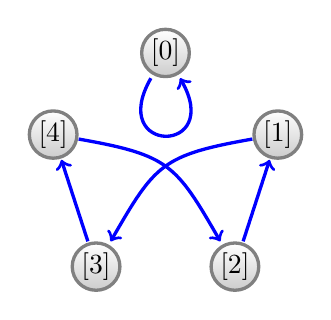
\begin{tikzpicture}[every node/.style={rectangle,minimum size=6mm,rounded corners=3mm,very thick,draw=black!50,top color=white,bottom color=black!20}]
  \node (A0) at (90:1.5) {$[0]$};
  \node (A1) at (90-72:1.5) {$[1]$};
  \node (A2) at (90-72*2:1.5) {$[2]$};
  \node (A3) at (90+72*2:1.5) {$[3]$};
  \node (A4) at (90+72:1.5) {$[4]$};
  \draw[very thick,blue,->] (A0) .. controls +(-120:1.5) and +(-60:1.5) .. (A0);
  \draw[very thick,blue,->] (A2) -- (A1);
  \draw[very thick,blue,->] (A3) -- (A4);
  \draw[very thick,blue,->] (A4) .. controls +(-10:1.5) and +(120:1.5) .. (A2);
  \draw[very thick,blue,->] (A1) .. controls +(190:1.5) and +(60:1.5) .. (A3);
\end{tikzpicture}%
}
Изобразим остатки по модулю $m$ точками, зафиксируем какой-либо остаток
$\alpha$ и из каждого остатка $\omega$ проведём стрелку в точку из $\omega$ в $\alpha\cdot \omega$.
Нарисуйте все такие картинки при $m=6$ и $m=7$. (На рисунке дан пример для $m=5$ при $\alpha=3$.)
\кзадача



\ВосстановитьГраницы


\задача Приведите пример, когда произведение двух ненулевых остатков по модулю $m$ является нулевым остатком. Такие остатки
называют \выд{делителями нуля}.
\кзадача

\задача Докажите, что натуральное число $m$ простое если и только если
среди остатков по модулю $m$ нет делителей нуля.
\кзадача

\опр Остаток $\beta$ называется  \выд{обратным} (по умножению) к остатку $\alpha$ по модулю $m$, если $\alpha\cdot\beta \equiv 1 \pmod{m}$.
Остаток, к которому имеется обратный, называется \выд{обратимым} (по умножению).
\копр

\задача
Докажите, что ненулевой остаток не является делителем нуля по некоторому модулю $m$ если и только если он обратим.
\кзадача

\задача \пункт Докажите, что целое $m > 1$ простое если и только если
для любого ненулевого остатка по модулю $m$ найдётся обратный к нему остаток по модулю $m$.
\пункт Докажите, что он единствен.
\кзадача

\задача
Пусть $p$ --- простое число.\\
%\сНовойСтроки
\вСтрочку
\пункт Найдите все такие $\alpha$ из $\Z_p$, что $\alpha^2=[1]$
(то есть $\alpha$ обратен (по умножению) сам себе).\\
\пункт Чему равно произведение всех ненулевых элементов $\Z_p$?
\кзадача

\задача {\it (Критерий Вильсона)}
%\footnote[1]{Александр Вильсон (1714 -- 1786) --- шотландский астроном и математик-любитель.}.)}
%профессор астрономии в Глазго.}.)}
Докажите, что целое число $m>1 $ простое тогда и только тогда, когда $(m-1)!+1\equiv0\!\pmod{m}$.
\кзадача

\задача %{\it (Малая теорема Ферма)}
%\footnote[2]{Пьер Ферма (1602 -- 1665) --- великий французский математик, один из основоположников теории чисел.}.)}
Пусть $p$ --- простое, $\alpha\in\Z_p$, $\alpha\ne[0]$.\\
\пункт
Домножим все элементы $\Z_p$ на $\alpha$. Докажите, что снова получатся
все элементы $\Z_p$.\\
\пункт
%Докажите, что $a^{p-1}\equiv1\!\pmod{p}$.
Выведите из пункта а) {\it малую теорему Ферма}: $\alpha^{p-1}=[1]$.
%\пункт
%Докажите, что $b^{p}\equiv b\!\pmod{p}$ при любом целом $b$.
\кзадача



